\documentclass{article}
\usepackage[margin=.5in]{geometry}
\usepackage{graphicx, dblfloatfix}
\usepackage{amsmath, amssymb, amsfonts, mathrsfs, mathtools, physics}
\usepackage[english]{babel}
\usepackage[autostyle, english = american]{csquotes}
\usepackage[normalem]{ulem}
\usepackage[title,titletoc,toc]{appendix}
\usepackage{pgfplotstable}
\usepackage{array, booktabs, colortbl, caption}
\MakeOuterQuote{"}

\title{Parity of Positroium}
\author{Alejandro Legarda}

\begin{document}
\raggedright
\maketitle

\begin{abstract}
We investigate the photons produced in positronium decay to confirm the conservation of parity through the decay. We expect, due to conservation laws, that photons will be emitted by the decay in orthogonally plane-polarized configurations. We use this and the fact that photons preferentially scatter in the direction orthogonal to their plane polarization during Compton scattering to show evidence of odd parity in the two-photon system, and hence conservation for the whole decay.
\end{abstract}

\tableofcontents
\newpage


\section{Theory}
Poitronium is a meta-stable particle composed of an electron and a positron in a


\section{Method}

\begin{figure}[!htb]
	\centering
	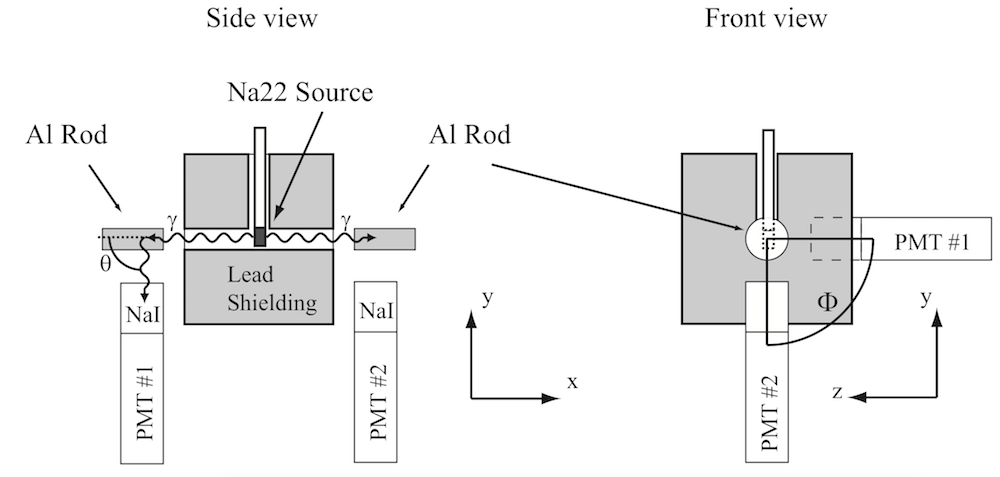
\includegraphics[scale=0.5]{apparatus.png}
  	\caption{The experimental apparatus. A Na-22 source is housed inside lead shielding. Aluminum rods are aligned with the openings of the shielding, which Compton scatter photons into the photomultiplier tubes.} 
 	\label{Apparatus}
\end{figure}